\documentclass[11pt,twocolumn]{article}
\usepackage{caption}
\usepackage{anysize}
\usepackage{fancyhdr}
\usepackage{graphicx}
\usepackage{subcaption}
\usepackage{color}
\usepackage{balance}
\usepackage{lipsum}
\usepackage{multirow}
\usepackage{multicol}

\marginsize{.75in}{.75in}{.75in}{1in}
\pagestyle{fancy}
\rhead{\today}
\lhead{
\includegraphics[height=2.0cm]{logo.jpg}}
\rfoot{\thepage}
\cfoot{}
\renewcommand{\headrulewidth}{0pt} %removes line from fancy header
\renewcommand{\thispagestyle}[1]{} %placers header and footer on first page 
\renewcommand{\abstractname}{Summary}
\setlength{\columnsep}{25pt}
\date{}
\title{Laboratory Gasification Memo\\Mixing Cup Temperature Experiments}

\begin{document}

\twocolumn[
  \begin{@twocolumnfalse}
    \maketitle
    \begin{abstract}
    
    An experimental campaign has been completed which explored the effect of inlet reactant temperature on biomass gasification. Space times were varied between 1.5 and 3.0 seconds, and mixing cup
temperatures of the reactants were varied between 168 and 281 $^\circ$C. Initial analyses suggest that higher
mixing cup temperatures led to increased conversion to carbon monoxide and carbon dioxide as well
as lower methane production.

    \end{abstract}
  \end{@twocolumnfalse}
]

\section*{Experimental Methods}

This experimental campaign was designed as a
two factor full factorial which examines two levels each of mixing cup temperature set point and
space time. Two replicates of the experimental
matrix were run to give sufficient statistical power
to limit the risk of not detecting differences in
means of 4\% in the measured CO and CO$_2$ yield.
A center point was run and replicated three times
estimate variance in results.

Steam to biomass, CO$_2$ to biomass, and argon
to biomass ratios were kept the same through-
out the experimental campaign. Inlet steam temperature and total nitrogen flow were changed to
match desired mixing cup temperatures and space
times given in Table \ref{mix_sp}. In calculating the mixing cup temperature, adiabatic mixing between
the species in the gas phase in all reactor inlets
were assumed. Because of the difficulty in estimating the rate of heat transfer between the solid
biomass and hot steam right at the exit of the lance as it enters the hot reactor, the heat capacity of biomass is not accounted for in these calculations. This means the mixing cup temperatures calculated in this report are likely somewhat
higher than actuality.

\begin{table}
	\centering
	\caption{Setpoints for mixing cup temperature and space time explored in the experimental campaign.}
	\label{mix_sp}
	\begin{tabular}{c c}
	Mixing Cup Temp	&	Space Time	\\
	K				&	seconds		\\
	\hline
	554				&	1.5			\\
	554				&	1.5			\\
	498				&	2.2			\\
	441				&	3.0			\\
	441				&	3.0			\\
	\end{tabular}
\end{table}

Reactor outer wall temperature was varied between 1350 $^\circ$C and 1450 $^\circ$C, and pressure was 50 psig for all experiments. Feedstock was ≤ 250 $\mu$m dry Southern yellow pine SEP. At the time
of writing this memo, duplicates for 1.5 second
experiments as well as a midpoint run were yet
to be completed at 1350 $^\circ$C. Detailed set points
of interest for each experiment can be found in
Appendix A. Biomass properties for each run are
given in Appendix B.

Four main results are discussed in this memo.
The first is total conversion, denoted as X$_{tot}$ in
Equation \ref{eq_total}. This is a measure of the fraction of
carbon in the biomass which is converted to any
gaseous product. The carbon in the entrainment
CO$_2$ is corrected for in the inlet and outlet so that
unreacted CO$_2$ does not contribute to conversion
totals.

\begin{equation}
	X_{tot} = \frac{\dot{n}_{C out,gas} - \dot{n}_{C_{in,CO_2}}}{\dot{n}_{C in,biomass}}
	\label{eq_total}
\end{equation}

Good conversion, X$_{good}$ in Equation \ref{eq_good}, is a measure of the fraction of carbon in the biomass which
is converted to either CO or CO$_2$ .

\begin{equation}
	X_{tot} = \frac{\dot{n}_{C out,CO} + \dot{n}_{C out,CO_2}- \dot{n}_{C_{in,CO_2}}}{\dot{n}_{C in,biomass}}
	\label{eq_good}
\end{equation}

Methane yield is denoted as Y$_{CH_4}$ in Equation
\ref{eq_ch4}. This equation calculates the fraction of carbon
in the biomass which is converted to methane.

\begin{equation}
	Y_{CH_4} = \frac{\dot{n}_{C out,CH_4}}{\dot{n}_{C in,biomass}}
	\label{eq_ch4}
\end{equation}

Finally, tar load is given in Equation \ref{eq_tar}. It is a
representation of the mass of benzene, toluene,
and naphthalene measured in the outlet gas.
$\dot{V}_{gas,out}$ is the volumetric flow rate of gas in standard cubic meters.

\begin{equation}
	Tar Load = \frac{\dot{m}_{C_6H_6} + \dot{m}_{C_7H_8}+ \dot{m}_{C_{10}H_8}}{\dot{V}_{gas,out}}
	\label{eq_tar}
\end{equation}

\section*{Results and Discussion}

\subsection*{Conversion}

Total and good conversion results from the experiments completed are shown in Figures \ref{plot_total} and \ref{plot_good},
respectively. A linear model was fitted to the results using a least squares fit with space time and
mixing cup temperature as parameters, as well as
an interaction effect term between the two. The
plots show that higher mixing cup temperatures
lead to higher conversion rates at similar space
times.

\begin{figure*}
	\centering
	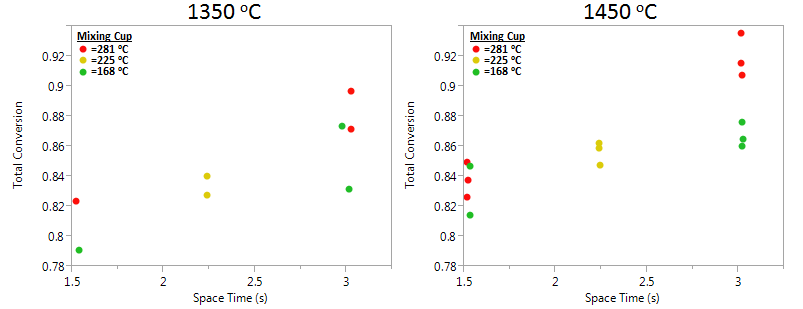
\includegraphics[width = \textwidth]{x_tot.png}
	\caption{}
	\label{plot_total}
\end{figure*}

\begin{table}
	\centering
	\caption{Effect significance for total conversion.}
	\label{tbl_total}
	\begin{tabular}{|c|c|c|}
	\hline
	T ($^\circ$C)			&	Effect				&	Prob \textless F	\\
	\hline
	\multirow{3}{*}{1350}	&	Space Time			&	\color{red}{0.0176} \\
	{}					&	Mixing Cup			&	0.1119 \\
	{}					&	Space Time * Mixing Cup	&	0.9425 \\
	\hline
	\multirow{3}{*}{1450}	&	Space Time			&	\color{red}{\textless 0.0001} \\
	{}					&	Mixing Cup			&	\color{red}{0.0018} \\
	{}					&	Space Time * Mixing Cup	&	\color{red}{0.0159} \\	
	\hline
	\end{tabular}
\end{table}

\begin{figure*}
	\centering
	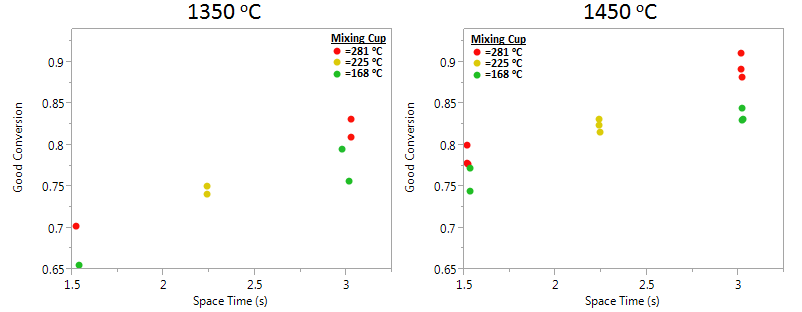
\includegraphics[width = \textwidth]{x_good.png}
	\caption{}
	\label{plot_good}
\end{figure*}

\begin{table}
	\centering
	\caption{Effect significance for good conversion.}
	\label{tbl_good}
	\begin{tabular}{|c|c|c|}
	\hline
	T ($^\circ$C)			&	Effect				&	Prob \textless F	\\
	\hline
	\multirow{3}{*}{1350}	&	Space Time			&	\color{red}{0.0015} \\
	{}					&	Mixing Cup			&	\color{red}{0.0391} \\
	{}					&	Space Time * Mixing Cup	&	0.8446 \\
	\hline
	\multirow{3}{*}{1450}	&	Space Time			&	\color{red}{\textless 0.0001} \\
	{}					&	Mixing Cup			&	\color{red}{0.0001} \\
	{}					&	Space Time * Mixing Cup	&	0.051 \\	
	\hline
	\end{tabular}
\end{table}

Different models were fitted to each set of experiments run at 1350 $^\circ$C and 1450 $^\circ$C. While the
conversions may not necessarily be a linear function of space time and mixing cup temperature,
running ANOVA on the effects can give a good
indication of which effects have statistical significance on the conversions. Table \ref{tbl_total} gives results
for total conversion, and Table \ref{tbl_good} gives results for
good conversion. Effects which had statistical significance using an alpha of 0.05 are highlighted in
red.

For total conversion, the mixing cup temperature does not have a statistically significant impact on total conversion at 1350 $^\circ$C, while it does
have an impact on total conversion for experiments run at 1450 $^\circ$C. However, mixing cup temperature affects the good conversion results for
both 1350 $^\circ$C and 1450 $^\circ$C.

\subsection*{Methane Yield}

Methane yield is calculated as the fraction of carbon in the biomass that is converted into methane
in the product stream. Figure \ref{plot_ch4} shows that
higher mixing cup temperatures may lead to lower
methane yields at each 1350 $^\circ$C and 1450 $^\circ$C. Running tests to detect statistical significance on the
same parameters as before shows that there is a
significant effect on methane yield from the mixing cup temperature at 1350 $^\circ$C but not at 1450
$^\circ$C.  However, it's important to note that the probability that there is an impact from mixing cup
temperature is very close to the alpha value of
0.05 in both cases. Thus, we can conclude that the
mixing cup temperature has an effect on methane
yield at both temperatures with about a 95\% certainty.

\begin{figure*}
\centering
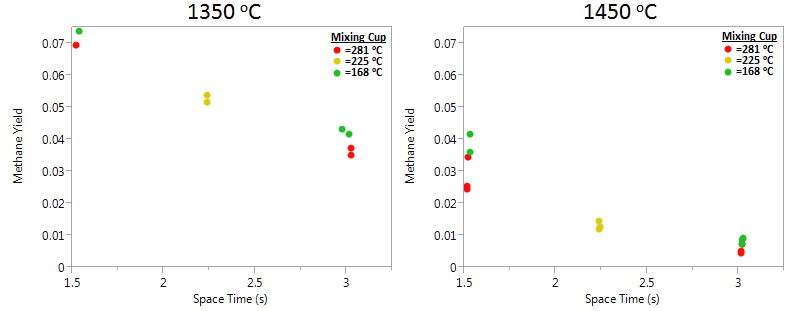
\includegraphics[width = \textwidth]{ch4_yield.png}
\caption{}
\label{plot_ch4}
\end{figure*}

\begin{table}
	\centering
	\caption{Effect significance for methane yield}
	\label{tbl_ch4}
	\begin{tabular}{|c|c|c|}
	\hline
	T ($^\circ$C)			&	Effect				&	Prob \textless F	\\
	\hline
	\multirow{3}{*}{1350}	&	Space Time			&	\color{red}{\textless 0.0001} \\
	{}					&	Mixing Cup			&	\color{red}{0.0495} \\
	{}					&	Space Time * Mixing Cup	&	0.8322 \\
	\hline
	\multirow{3}{*}{1450}	&	Space Time			&	\color{red}{\textless 0.0001} \\
	{}					&	Mixing Cup			&	0.0530 \\
	{}					&	Space Time * Mixing Cup	&	0.2476 \\	
	\hline
	\end{tabular}
\end{table}

\subsection*{Tar Loading}

Tar loading is expressed as the mass of tar in mg
in a standard cubic meter of gas. Figure \ref{plot_tar} shows
results from the experiments. Note that the y-axis for each plot is on a different scale, and the
tar levels at 1450 $^\circ$C are much lower than those
at 1350 $^\circ$C. This is a typical difference based on
previous experiments run at these temperatures.
Table \ref{tbl_tar} shows that there is not a statistically
significant effect on tar loading from the mixing
cup temperature. However, the tar levels at 1450
$^\circ$C are already so low that any differences may
be hard to detect on our system. Also, longer
space times at 1350 $^\circ$C have historically showed
lower tar loadings. It would be interesting to revisit these results once the 1.5 second space time
replicate experiments are completed at 1350 $^\circ$C to
see if a difference is detected at the shorter space
time.

\begin{figure*}
\centering
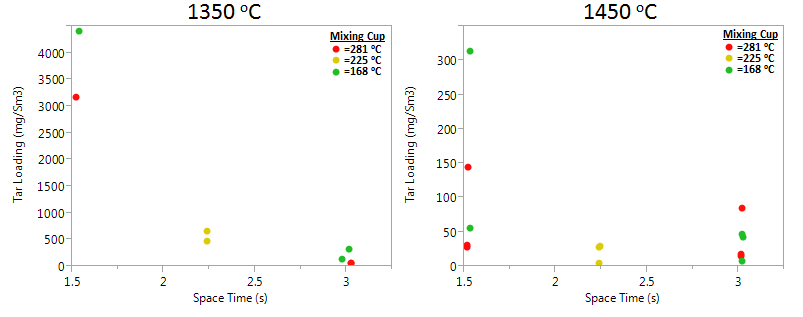
\includegraphics[width = \textwidth]{tar_loading.png}
\caption{}
\label{plot_tar}
\end{figure*}

\begin{table}
	\centering
	\caption{Effect significance for tar loading.}
	\label{tbl_tar}
	\begin{tabular}{|c|c|c|}
	\hline
	T ($^\circ$C)			&	Effect				&	Prob \textless F	\\
	\hline
	\multirow{3}{*}{1350}	&	Space Time			&	\color{red}{0.0114} \\
	{}					&	Mixing Cup			&	0.4719 \\
	{}					&	Space Time * Mixing Cup	&	0.4841 \\
	\hline
	\multirow{3}{*}{1450}	&	Space Time			&	0.0988 \\
	{}					&	Mixing Cup			&	0.3054 \\
	{}					&	Space Time * Mixing Cup	&	0.2320 \\	
	\hline
	\end{tabular}
\end{table}

\section*{Conclusion}

The experimental campaign explored the effects
of mixing cup temperature at the inlet to the reactor for selected space times. Higher mixing cup
temperatures led to a higher good conversion at
both 1350 $^\circ$C as well as 1450 $^\circ$C. While lower
methane yields may be attributed to higher mixing cup temperatures, effects on tar loading are
not detected. Further exploration of shorter space
time ranges which are known to produce significant tars may reveal an effect on tar loading and
may even give more light to the magnitude of the
effect on methane yield at these space times, as
well.
\balance

\onecolumn
\appendix
\section{Experimental Set Points}
\label{app_sp}

\begin{center}
\begin{tabular}{ccccccccc}
	Run ID &  Temp 		&  Biomass 	&  Steam 	&  Steam 		&  Entrainment & Downbed	 & 	Makeup	&	Argon \\
	{}       & $^\circ$C	& lbs/hr		& ml/min	& $^\circ$C	& SLPM N$_2$	& SLPM CO$_2$	 & 	SLPM N$_2$ & SLPM \\
	\hline
	473    &       1450 &             4 &     24.16 &       500 &       24.16 &               6.60 &            0 &         2.0 \\
	474    &       1450 &             2 &     12.08 &       500 &       12.08 &               3.30 &            0 &         1.0 \\
	476    &       1450 &             2 &     12.08 &       350 &       12.08 &               3.30 &            8 &         1.0 \\
	477    &       1450 &             3 &     18.12 &       400 &       18.12 &               4.95 &            0 &         1.5 \\
	478    &       1450 &             2 &     12.08 &       500 &       12.08 &               3.30 &            0 &         1.0 \\
	479    &       1450 &             4 &     24.16 &       350 &       24.16 &               6.60 &           16 &         2.0 \\
	481    &       1450 &             2 &     12.08 &       350 &       12.08 &               3.30 &            8 &         1.0 \\
	482    &       1450 &             3 &     18.12 &       400 &       18.12 &               4.95 &            0 &         1.5 \\
	484    &       1450 &             4 &     24.16 &       500 &       24.16 &               6.60 &            0 &         2.0 \\
	489    &       1450 &             4 &     24.16 &       350 &       24.16 &               6.60 &           16 &         2.0 \\
	490    &       1450 &             3 &     18.12 &       400 &       18.12 &               4.95 &            0 &         1.5 \\
	495    &       1450 &             4 &     24.16 &       500 &       24.16 &               6.60 &            0 &         2.0 \\
	496    &       1450 &             2 &     12.08 &       350 &       12.08 &               3.30 &            8 &         1.0 \\
	497    &       1450 &             2 &     12.08 &       500 &       12.08 &               3.30 &            0 &         1.0 \\
	500    &       1350 &             4 &     24.16 &       500 &       24.16 &               6.60 &            0 &         2.0 \\
	501    &       1350 &             2 &     12.08 &       500 &       12.08 &               3.30 &            0 &         1.0 \\
	502    &       1350 &             3 &     18.12 &       400 &       18.12 &               4.95 &            0 &         1.5 \\
	503    &       1350 &             4 &     24.16 &       350 &       24.16 &               6.60 &           16 &         2.0 \\
	504    &       1350 &             2 &     12.08 &       350 &       12.08 &               3.30 &            8 &         1.0 \\
	505    &       1350 &             2 &     12.08 &       500 &       12.08 &               3.30 &            0 &         1.0 \\
	506    &       1350 &             2 &     12.08 &       350 &       12.08 &               3.30 &            8 &         1.0 \\
	507    &       1350 &             3 &     18.12 &       400 &       18.12 &               4.95 &            0 &         1.5 \\
	508    &       1350 &             4 &     24.16 &       350 &       24.16 &               6.60 &           16 &         2.0 \\
	509    &       1350 &             3 &     18.12 &       400 &       18.12 &               4.95 &            0 &         1.5 \\
	510    &       1350 &             4 &     24.16 &       500 &       24.16 &               6.60 &            0 &         2.0 \\
\end{tabular}
\end{center}

\pagebreak

\section{Biomass Properties}
\label{app_bm}

\begin{center}
\begin{tabular}{ccc}
	Run ID	&	Moisture	&	Carbon	\\
	{}		&	\% wt	&	\% wt	\\
	\hline
	473    &      7.20 &  54.06 \\
	474    &      7.20 &  54.06 \\
	475    &      7.20 &  54.06 \\
	476    &      7.20 &  54.06 \\
	477    &      7.20 &  54.06 \\
	478    &      7.20 &  54.06 \\
	479    &      7.20 &  54.06 \\
	480    &      7.20 &  54.06 \\
	481    &      7.20 &  54.06 \\
	482    &      7.20 &  54.06 \\
	484    &      7.20 &  54.06 \\
	489    &      7.49 &  54.06 \\
	490    &      7.20 &  54.06 \\
	495    &      6.68 &  54.06 \\
	496    &      6.68 &  54.06 \\
	497    &      7.49 &  54.06 \\
	500    &      6.94 &  54.06 \\
	501    &      8.61 &  54.06 \\
	502    &      8.61 &  54.06 \\
	503    &      6.94 &  54.06 \\
	504    &      7.49 &  54.06 \\
	505    &      8.61 &  54.06 \\
	506    &      8.61 &  54.06 \\
	507    &      8.61 &  54.06 \\
	508    &      7.49 &  54.06 \\
	509    &      6.94 &  54.06 \\
	510    &      6.93 &  54.06 \\
\end{tabular}
\end{center}

\section{Variable Definitions}
\begin{center}
	\begin{tabular}{rl}
	Variable Name			&	Description	\\
	\hline
	$\dot{m}_{C in,i}$		&	Mass flow rate of species i into the system.	\\
	$\dot{m}_{C out, i}$	&	Mass flow rate of species i out of the system.	\\
	$\dot{n}_{C in, i}$		&	Molar flow rate of carbon into the system in species i.	\\
	$\dot{n}_{C out, i}$		&	Molar flow rate of carbon out of the system in species i.	\\
	$\dot{n}_{C out, gas}$	&	Molar flow rate of carbon out of the system in all gaseous species.	\\
	$X_{good}$			&	Total conversion of carbon in biomass into gaseous species.	\\
	$X_{tot}$				&	Conversion of carbon in biomass to CO and CO2 .	\\
	$Y_{CH_4}$			&	Methane yield.	\\
	\end{tabular}
\end{center}

\end{document}

